\begin{figure}
    \begin{center}
    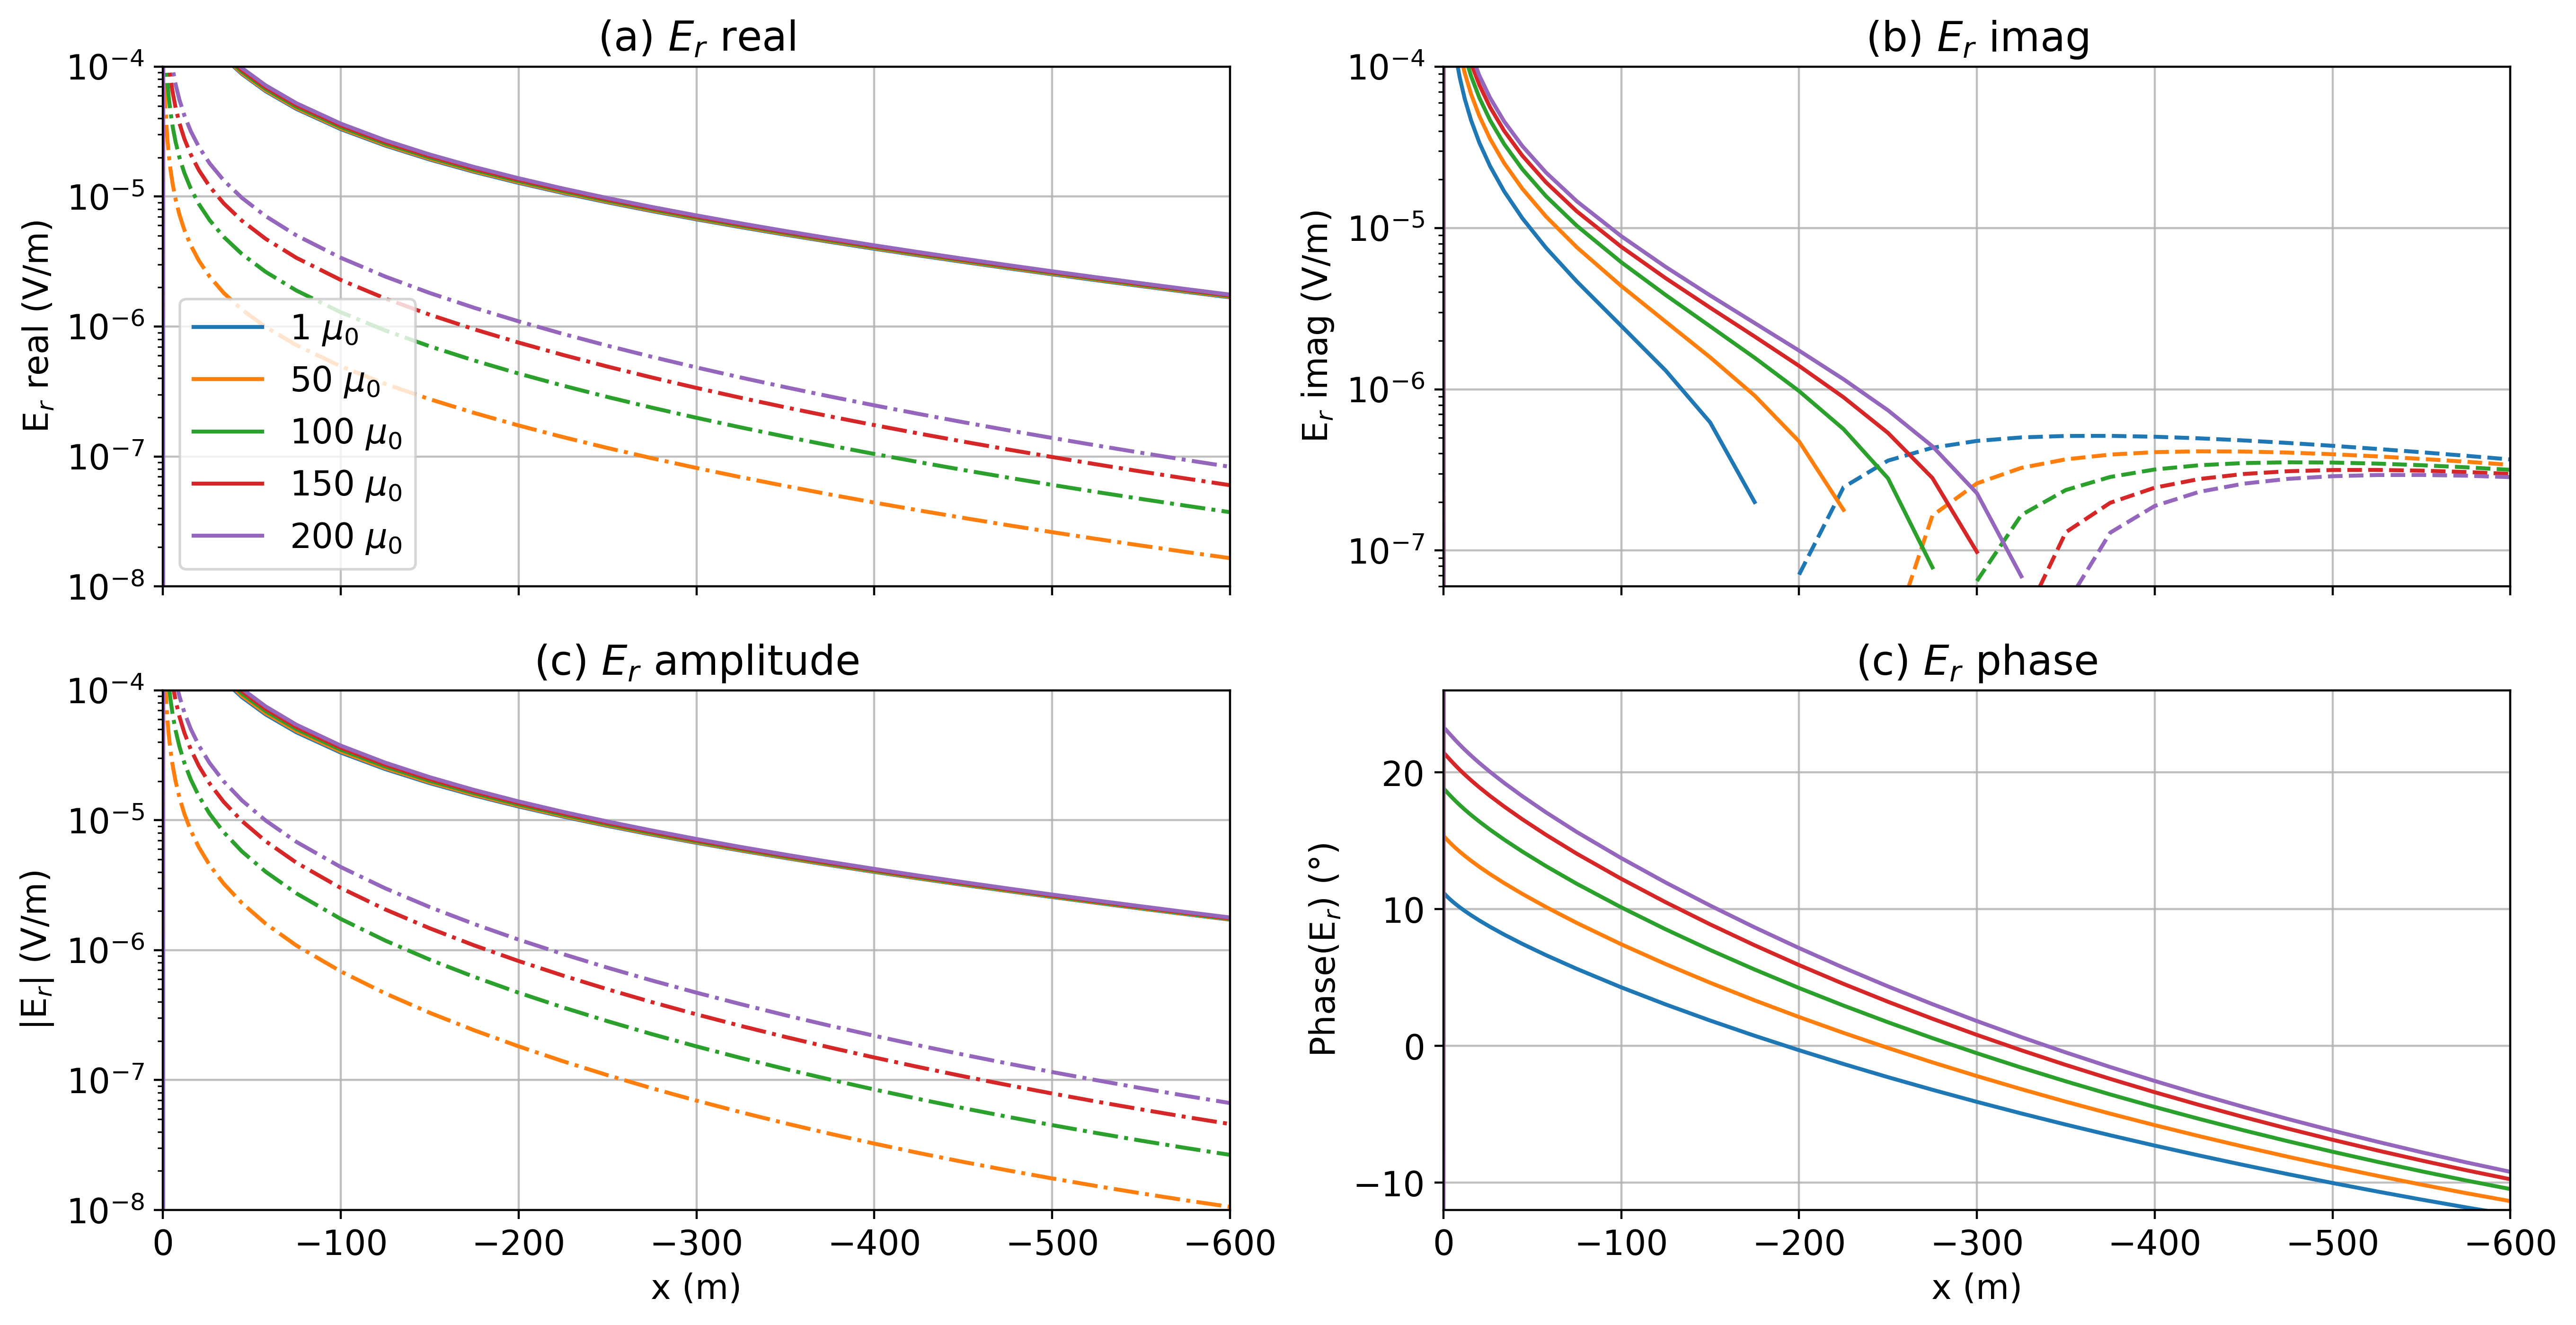
\includegraphics[width=\textwidth]{figures/e-fields-fdem.png}
    \end{center}
\caption{
    Radial electric field data for a top-casing experiment at 5Hz with the setup as shown in Figure \ref{fig:setup}. The top row shows (a) the real and (b) the imaginary components and the bottom row shows (c) the amplitude and (d) the phase. Solid lines indicate positive values (pointing away from the well) and dashed lines indicate negative values (pointing towards the well). In (a) and (c) we also show the difference between each of the permeable well scenarios and a non-permeable well ($\mu_r=1$) with the dash-dot lines.
}
\label{fig:e-fields-fdem}
\end{figure}



